% sections/02-predictive-optimistic-execution.tex

\section{Predictive optimistic execution}

We propose \textbf{Predictive Optimistic Execution}, an approach designed to enhance optimistic execution algorithms by predicting transaction dependencies with high accuracy. This method reduces conflict rates and boosts the efficiency of parallel executions.

Traditional optimistic execution algorithms face difficulties with high-conflict blocks, which will lead to a large amount of redundant execution of related transactions and a significant decline in the efficiency of parallel EVMs. 

Artela introduce an \textbf{optimistic execution methodology} (Figure \ref{fig:predictive_optimistic_execution}) complemented by a \textbf{prediction module}. This module proactively analyzes transaction dependencies based on hints associated with transactions and contracts, thereby forming execution groups for transactions to reduce the possible re-execution. A hint table is incorporated, which logs the state access information of transactions and contracts. The hint table serves as the input for the prediction algorithm; these hints are dynamically accumulated through analysis of historical transaction execution processes and do not require user input.

\begin{figure*}[htp]
\centering
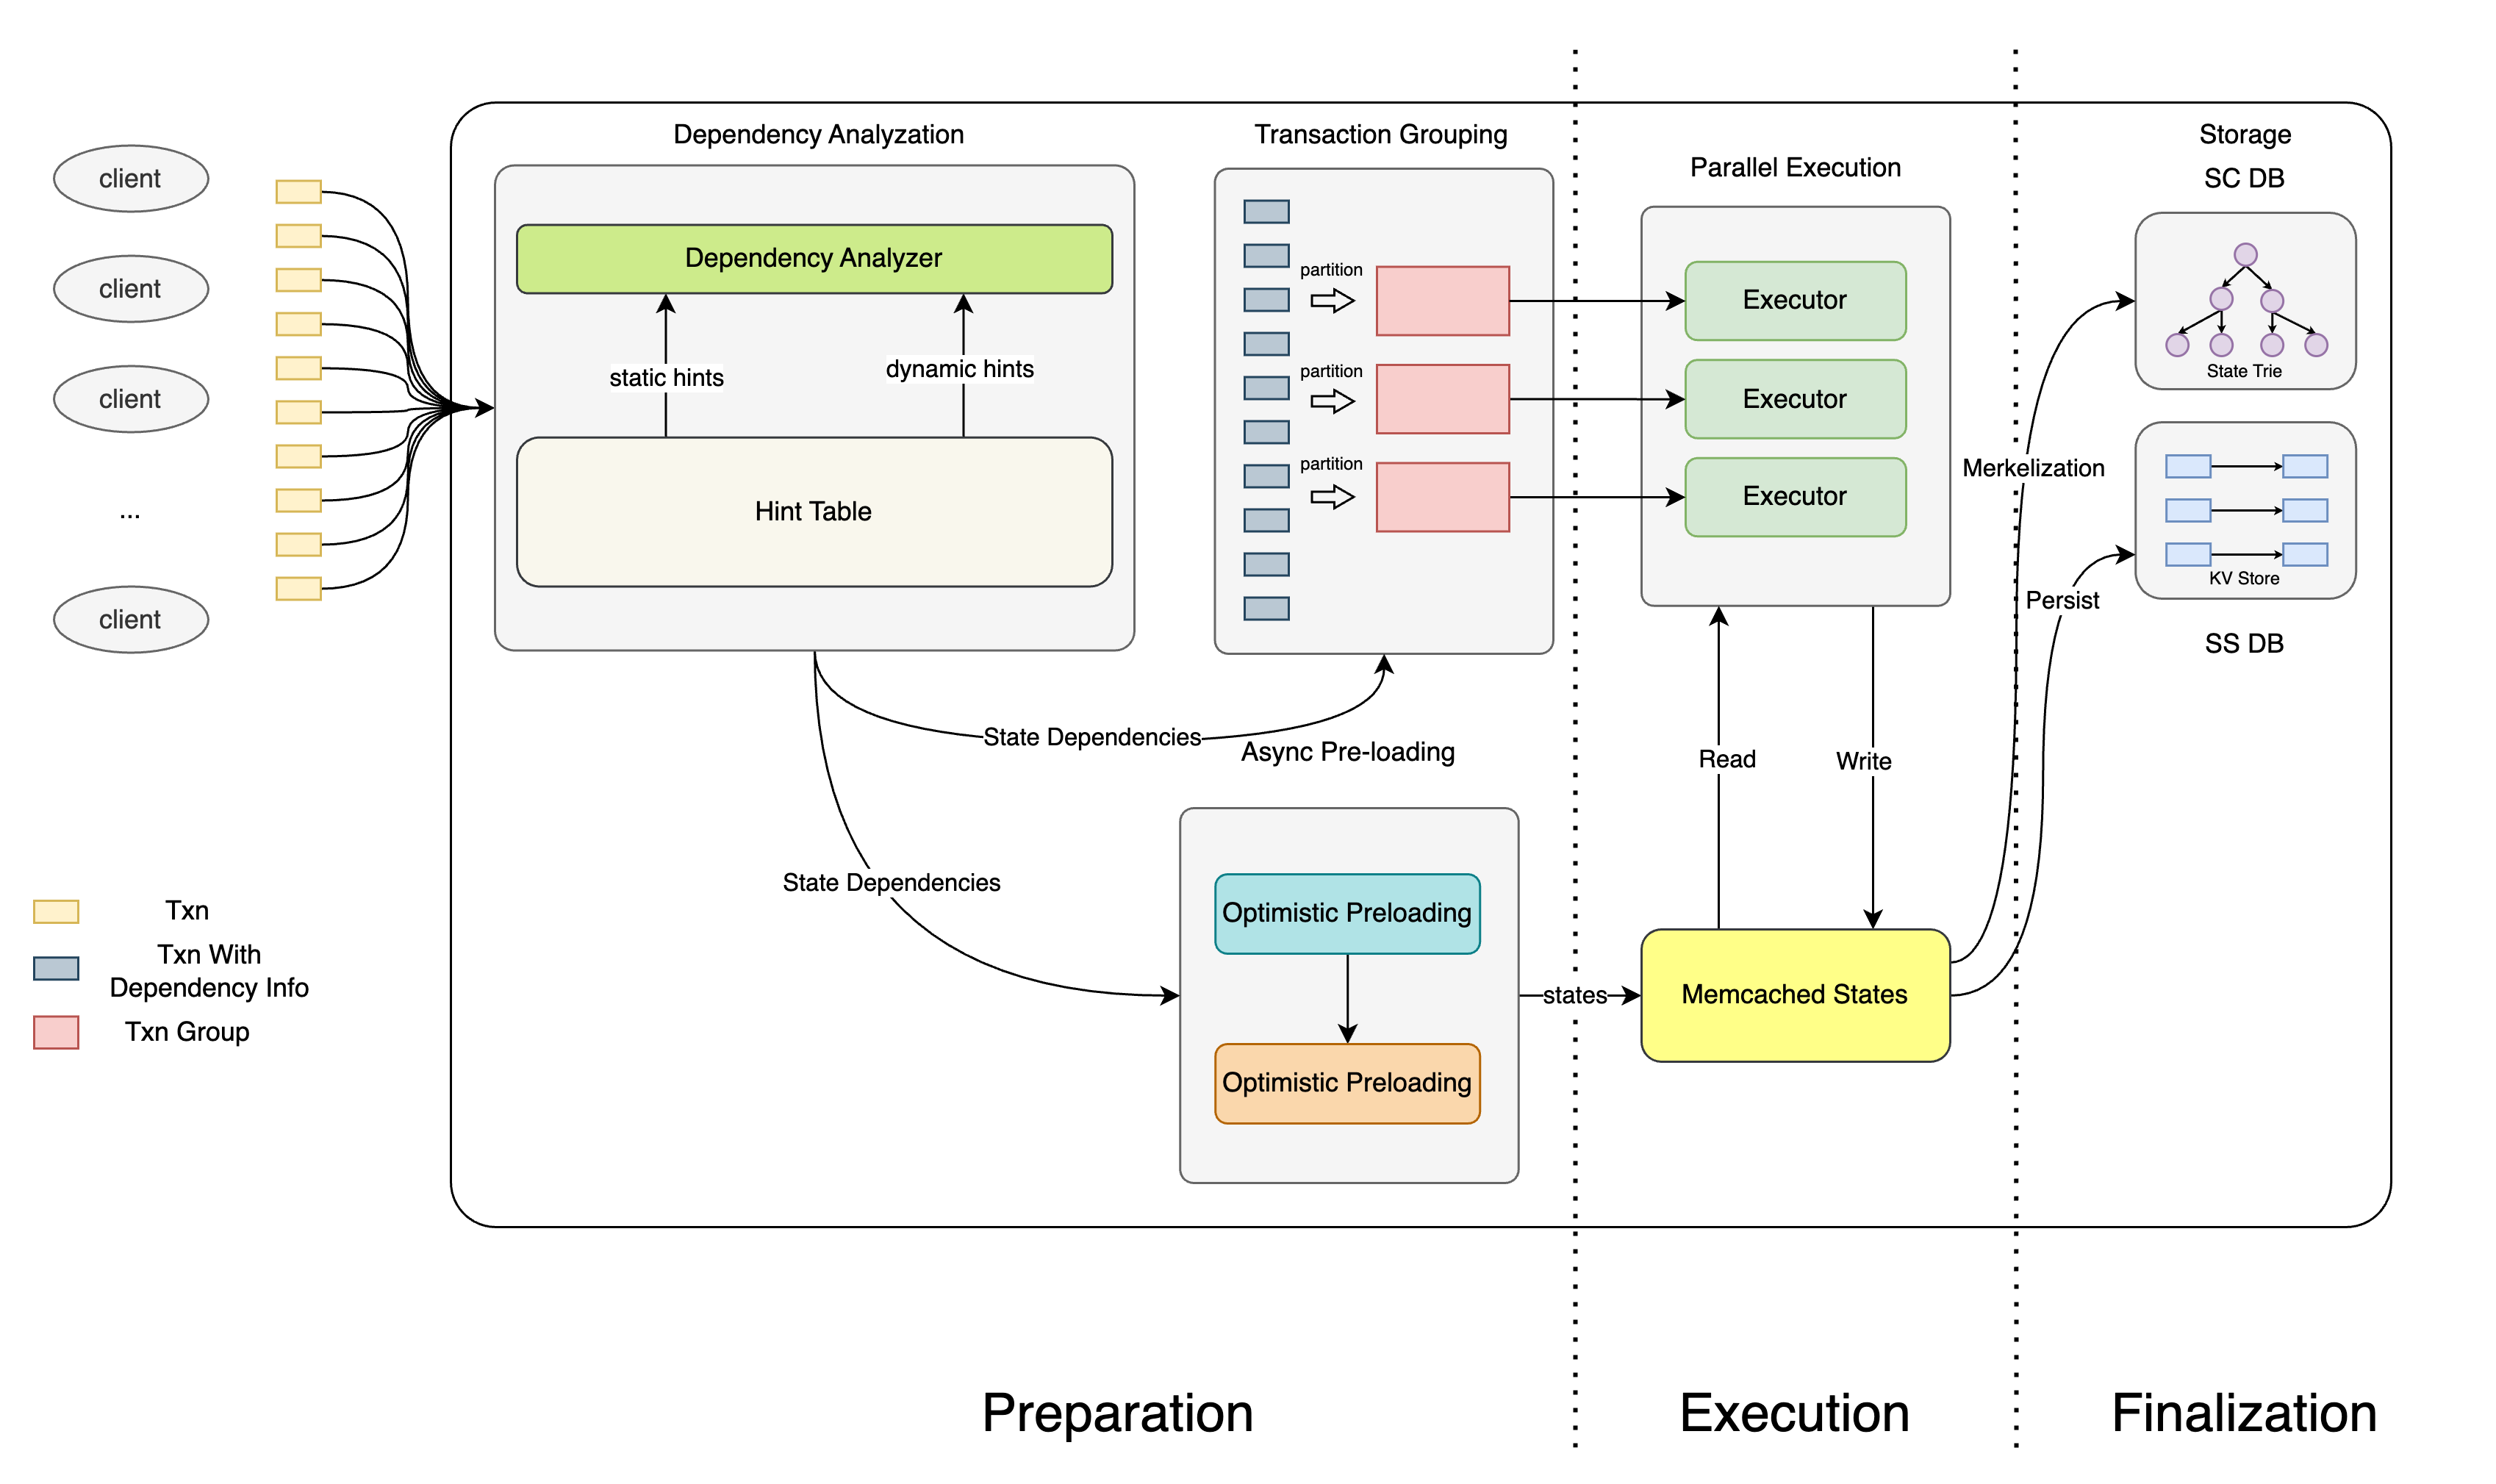
\includegraphics[width=0.75\textwidth]{sections/images/predictive-optimistic-execution.png}
\caption{Predictive Optimistic Execution}
\label{fig:predictive_optimistic_execution}
\end{figure*}

\subsection{Optimistic Execution}

The implementation of parallel execution lies in Optimistic Execution, a strategy where transactions are speculatively processed under the initial assumption that there are no conflicts. Each transaction maintains a private version of the state, recording modifications without immediate finalization. After the transaction is executed the transaction, a subsequent validation phase will examine for potential conflicts against global state alterations effected by concurrent transactions within the same interval. Any detected conflicts will result in the re-execution of the transaction. 

This approach leverages a multi-version data structure and upholds a pre-defined serialization order to ensure data consistency and integrity. The refinement of the optimistic execution algorithm will be integrated through enhancements in Block-STM\cite{gelashvili2022blockstm}.

\subsection{Hint table}

In this section, we will discuss the current challenges associated with existing hint resolution methods and discuss how \textbf{Artela's Hint Table} addresses these issues through its implementation.

\textbf{Hint Table} serves as an auxiliary database table. It is \textbf{persisted on the hard drive} and will be \textbf{preloaded into memory} prior to usage. The hint table cataloges potential transaction and contract read / write sets. This aids the division of transactions into parallel executable groups before execution, significantly reducing the conflict rate and re-execution times.

We will now discuss the current solutions similar to hint table and explain why they are inadequate for parallel execution needs.

\textbf{EIP-2930 (Optional Access Lists)\cite{buterin2020eip2930}.} EIP-2930 introducing the ability for users to submit their transactions' read and write sets, but since this is not mandatory, only a small fraction of transactions are using it (1.46\% until December 2023\cite{heimbach2023dissecting}) utilize this feature.

\textbf{Transaction Pre-Execution.} Transactions are initially sent to pre-execution nodes (non-Validator nodes), where these nodes collect potential read-write sets through pre-execution, a method fundamentally employed by systems such as Sui due to its cost-effectiveness. However, this approach necessitates the addition of protocols between non-Validator and Validator nodes within the network.

\textbf{Static Analysis.} This approach utilizes a compiler or other tools to conduct static analysis and abstract interpretation, identifying the potential read-write sets that contract execution may access. These are analyzed in advance and stored as static hints. Along with the contract's bytecode, these hints are sent to nodes. Before executing the contract, nodes load these hints to enhance static analysis. A significant drawback of this method is the requirement for developers to adhere strictly to conventions. Sending invalid hints can lead to issues during algorithm execution.

The Hint table is engineered to adeptly address distinct challenges associated with discovering transaction and contract read/write sets by leveraging a combination of static and dynamic analysis. The following is a detailed explanation of its implementation and strategic approach to resolving these challenges.

\subsubsection{Types of States}

The hint table will categorize the states of contracts into the following categories:

\textbf{Input-unrelated States:} These states are universally accessible and generally easier to be analyzed, for example the `totalSupply` state variable in an ERC20 contract.

\textbf{Input-related States:} These states are dynamic; they are typically associated with transaction data.
\begin{itemize}
\item \textbf{Account-related States:} Directly connected to specific accounts, these states relate to transaction fields like \textbf{`tx.from`} and \textbf{`tx.to`}.
\item \textbf{Miscellaneous States:} These are dynamically linked states whose relationships are not consistently determinable, often seen in complex contracts like Uniswap V4's \textbf{`positions`} mapping.
\end{itemize}
\subsubsection{Types of Hints}

Hints can be categorized into two types:

\textbf{Static Hints:} This type signifies a basic hint, typically used to suggest actions for input-unrelated states. We can represent this type of hints with the following symbols:
    
    \begin{equation}
    \[
    C(M) \Rightarrow \{ R(slot_i), W(slot_j), ..., R(slot_k) \}
    \]
    \end{equation}

    $C$ represents a set of static configurations, when a smart contract method $M$ gets called, corresponding storage slot $slot_i$ will be read ($R$) / write ($W$).
    
\textbf{Dynamic Hints:} This type signifies the complex hint, typically used to suggest actions for input-related states. Dynamic hints can be represented with the following symbols:
    
\begin{equation}
\begin{split}
    F_i(M, \{a_i, a_j, ..., a_k\}) \Rightarrow \{ &R(slot_i), \\
    &W(slot_j), \\
    &..., \\
    &R(slot_k) \}
\end{split}
\end{equation}
    
    This notation describes a more complex hint. Specifically, a given contract method $M$ has one or more input parameters that include accounts (denoted as $a$). The set ${a_i, a_j, ... , a_k}$ can be determined through a derivation algorithm $F_i$, which calculates the storage slots $slot_i$ accessed during the method's execution.
    
    Formed by analyzing historical execution data, dynamic hints adapt over time, enhancing their precision and relevance to current conditions.

\subsubsection{Hint Generation Process \& Format}

During transaction execution, the hint generation module captures and logs state accesses and contract calls for each method and contract address. 

Hints are structured in a key-value format where the key represents a combination of fields, and the value denotes a set of state slot indices. For input-related states, hints don’t log every storage slot but use a mapping function to represent them efficiently.

\subsubsection{Storage of Hints}

To ensure operational efficiency, hints are stored persistently but loaded entirely into memory when accessed. The total size of stored hints is capped at under 4GB to optimize memory usage and maintain system performance.

This comprehensive overview delineates the structure, generation, and utilization of hints within the system, which are integral to optimizing contract interactions and enhancing transaction processing efficiency. By categorizing and systematically managing hints, the system ensures high levels of accuracy and operational efficacy.

\subsection{AI-driven Hints Generator}

Unlike other solutions that require developers to manually generate hints, our approach automates the creation of the Hint table. Utilizing a specific AI model, this solution analyzes historical transaction data to automatically generate an accurate Hint table. This model operates off-chain, and the generated Hint table is synchronized with the network nodes. Additionally, the model can incorporate data from other EVM-compatible chains, leveraging similarities in protocols to enhance its accuracy.

Since the Hint table is updated based on historical data, initial transactions on the Artela blockchain may not benefit from high parallelism; a warm-up period is required. As the Hint table becomes more refined through ongoing updates, the parallelism of the chain will naturally improve.